\chapter{The GPU-based Implementation of DNA Recombination Algorithm}\label{Chapter:GPU}

We provide a detailed description regarding the GPU-based implementation of the DNA recombination algorithm in this chapter. We first evaluate two parallelization approaches for GPU-based implementation, and select the most suitable method based on their advantages and disadvantages in Section \ref{sec: Parallelization Strategy}. In Section \ref{sec:bitwise}, we propose the bit-wise GPU-based implementation for the DNA recombination algorithm. We extend the bit-wise implementation to a multi-GPU environment and provide a detailed explanation in Section \ref{sec:Multi-GPU}. Finally, we explain the experimental setup and simulation results for bit-wise implementation on a single and multi-GPU in Section \ref{sec:Multi-GPU} and \ref{sec:Result}, respectively.   
\section {The Parallelization Strategy}\label{sec: Parallelization Strategy}

In this section, we analyze two parallelization approaches for the GPU-based implementation of $V(D)J$ recombination process. For each strategy, we attempt to answer the following questions: 1) What would be the workload distribution based on the parallelization strategy? 2) Does the proposed parallelization strategy result in an even workload distribution among the threads? 


Since each $V-J$ pair generates a specific sequence, the first parallelization approach would be the $V-J$ level parallelism by assigning one $V$ gene, one $J$ gene, and both $D$ genes to each thread to perform the recombination process. In this assignment, each thread needs to cover all possible n-nucleotide lengths (zero to ten) along with all possible combinations of four bases for any given n-nucleotide lengths. However, as there are 20 $V$ genes and 12 $J$ genes, this implementation would require only 240 threads and result with significantly low thread utilization on the GPU. A finer granularity of $V-J$ level parallelism can be realized by assigning one form (refer to chewback and palindromic forms of each input gene) of $V$ gene, one form of $J$ gene, and both $D$ genes to each thread. For this approach, the total number of required threads is 102,446 since there are 362 $V$ genes, 283 $J$ genes in the chewback and palindromic forms for the mice data set.  This finer level of parallelization occupies 90\% of the threads on the target P100 series GPU. 

In order to answer the second question for the fine-grained $V-J$ level parallelization approach, we need to consider workload for both \emph{combination} and \emph{comparison} steps. We refer to the \emph{combination} step as a process of generating all possible \emph{in silico} sequences for a given input data and the \emph{comparison} step as a process of comparing generated sequences with \emph{in vivo} sequences. The workload distribution for \emph{combination} step is even since, each thread is assigned one form of $V$ gene, one form of $J$ gene, and both $D$ genes. In order to evaluate the workload distribution for the \emph{comparison} step, we provide a normalized distribution of \emph{in vivo} sequences across 240 $VJ$ pairs in Fig. \ref{fig:240PE}. As shown, total number of \emph{in vivo} sequences is not evenly distributed across different $VJ$ pairs, which directly affects the workload of each thread. Since, each thread needs to compare its generated \emph{in silico} sequences against every \emph{in vivo} sequence in the corresponding $VJ$ pair, the fine-grained $V-J$ based assignment results in an uneven workload distribution among GPU threads. 

\begin{figure}[t!]
\begin{center}
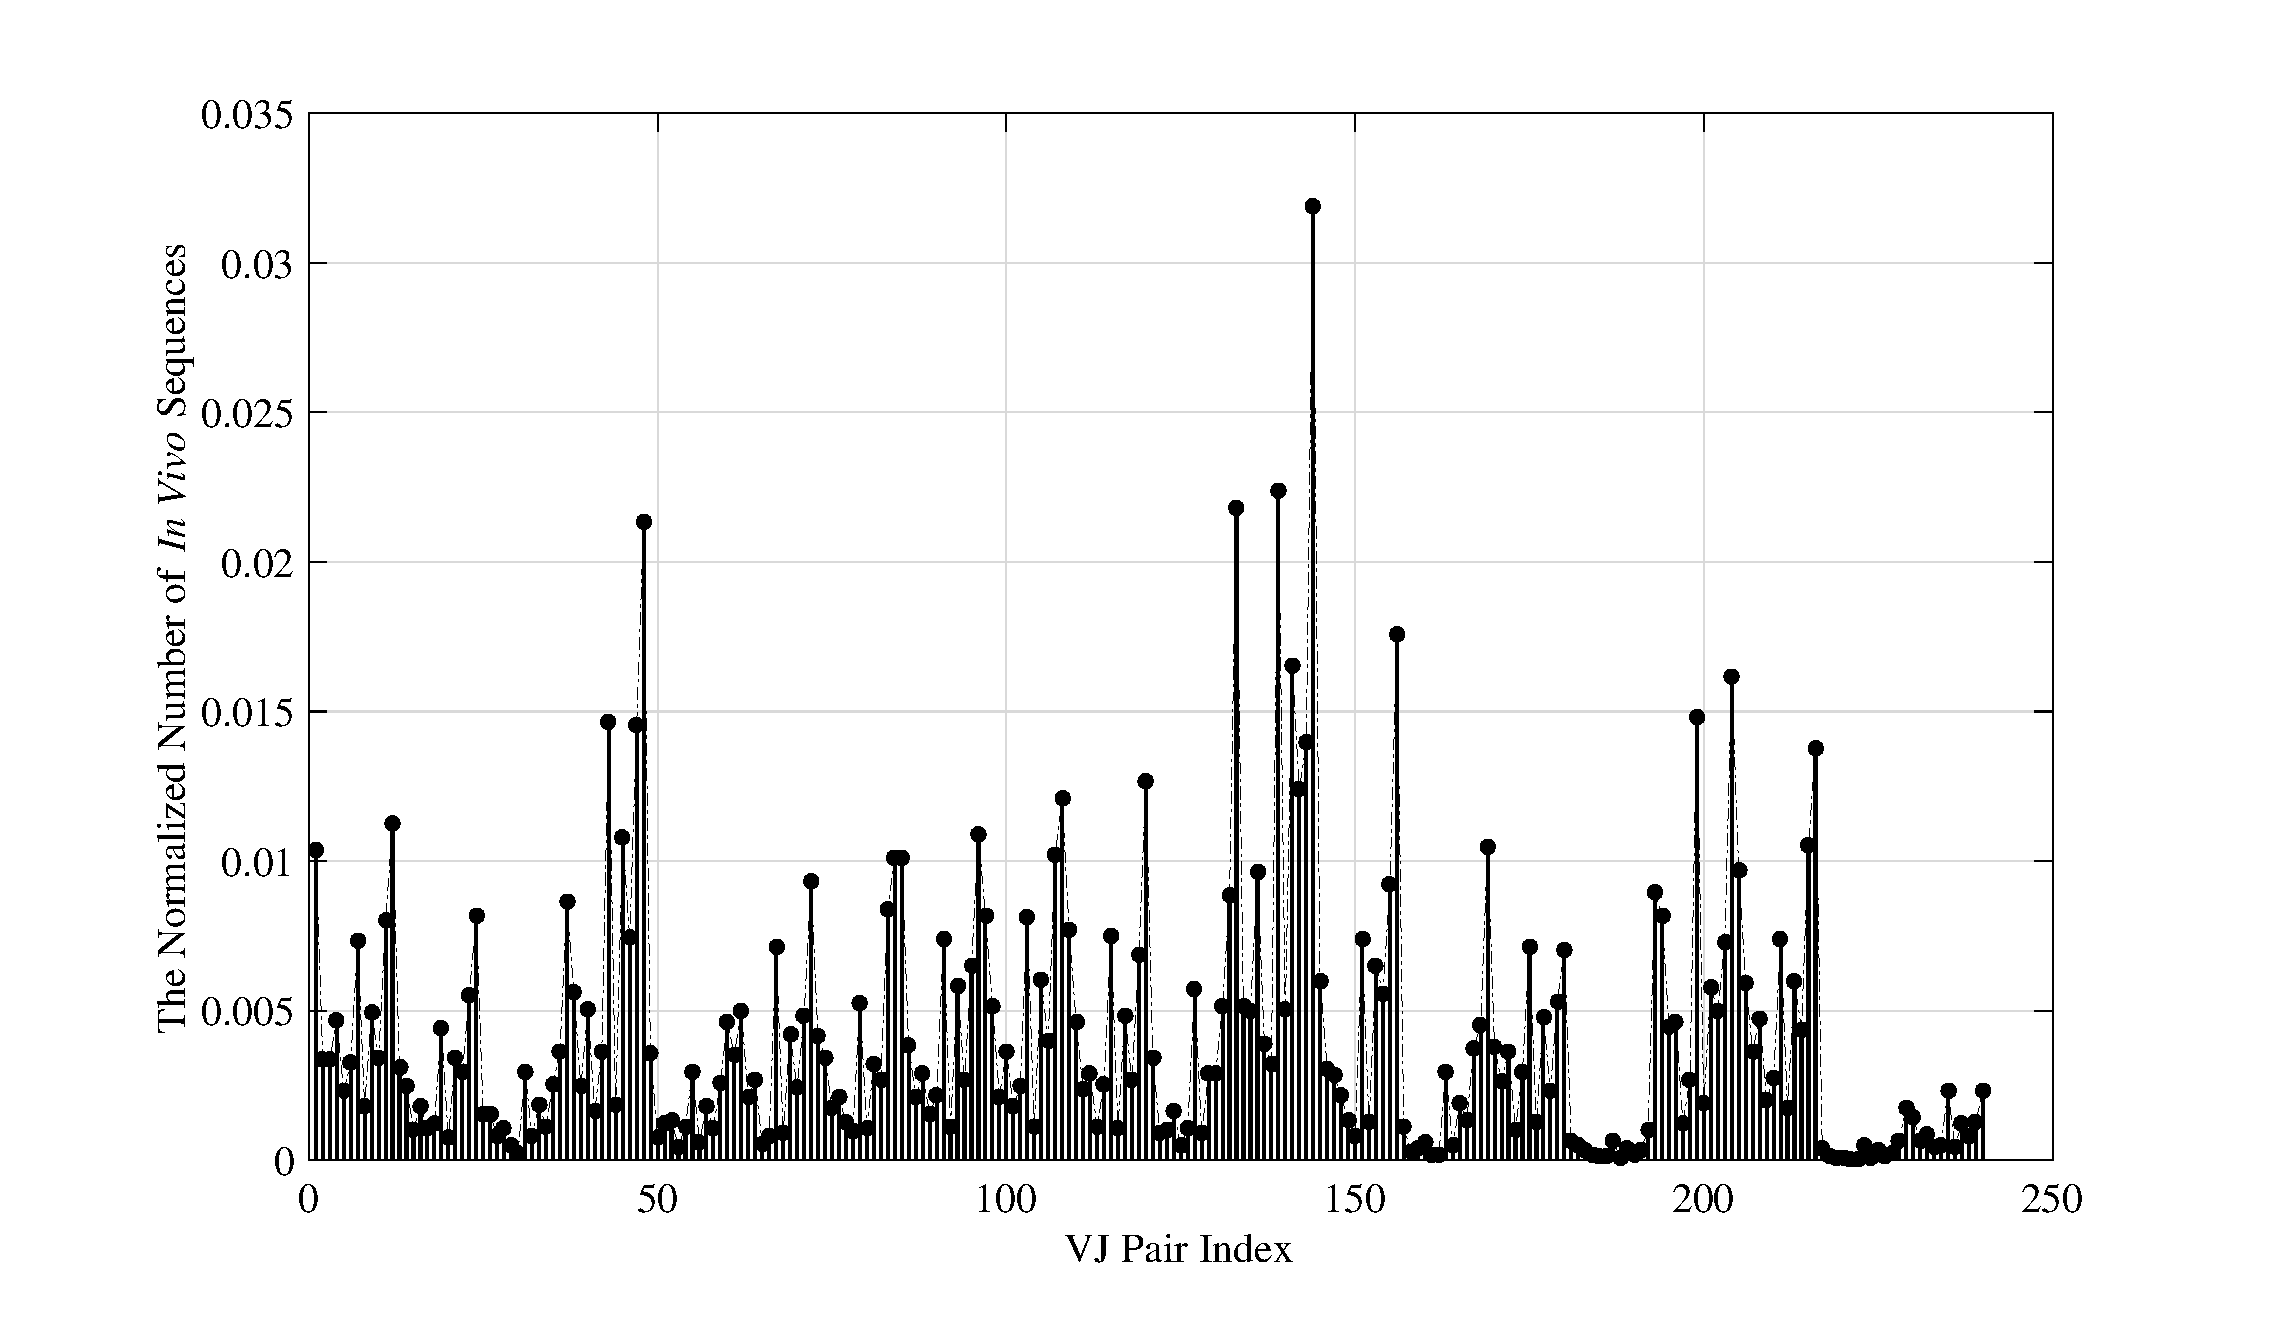
\includegraphics[clip,width=1\columnwidth]{Figure/1.eps}

\caption{ A Normalized distribution of \emph{in vivo} sequences across 240 VJ pairs.}
\label{fig:240PE}
\end{center}
\end{figure}


The second solution would be n-nucleotide level parallelism, where each thread is assigned a unique n-nucleotide sequence and the recombination process is applied on that unique sequence. In this assignment, the workload for the \emph{combination} step is even since, each thread works on one n-nucleotide sequence. In addition, the workload distribution for \emph{comparison} step is equal among GPU threads, since GPU threads are working on the same $V$ and $J$ gene. Therefore, total number of \emph{in vivo} sequence for the comparison process are equal among active threads. Since all threads share the same $V$ and $J$ gene pairs, this approach can take advantage of the shared memory to improve the the memory bandwidth utilization. 

In order to decide which one of the stated approaches performs better in terms of execution time, we evaluate the workload per thread for the \emph{combination} step, in both approaches. In the fine-grained $V-J$ level parallelism, each thread generates \emph{in silico} sequences for all possible forms of n-nuclotide for length of zero to ten. Table \ref{tab:n-table} shows the total number of n-nucleotide sequence based on the length. Therefore, a single thread must generate 706,042,015 \emph{in silico} sequences through the entire process as there are 1,381,717 unique n-nucleotide sequence in total and there are 505 sequences for $D$ gene. In the n-nucleotide based assignment, each thread generates 51,735,230 \emph{in silico} sequences since there are 362 $V$ genes, 283 $J$ genes, and 505 $D$ genes. As a result, workload per thread in fine-grained $V-J$ level parallelism is almost 13 times higher than n-nucleotide parallelization approach. In the following sections we present our approach to bit-wise and multi-GPU implementations based on n-nucleotide level parallelism. 



\begin{table}[t!]
\caption{The total number of unique n-nucleotide sequences based on the length of n-nucleotide}

\renewcommand{\arraystretch}{1.2}
\begin{center}
\begin{tabular}{ |c|c| }
  \hline
    \textbf{\textit{ N\_{len} }} & \textbf{\textit{Total number of unique}}\\
    ~ &  \textbf{\textit{n-nucleotide sequences}}\\	\hline	
    0 & 1  	\\	\hline
    1 & 4 		\\	\hline
   	2 & 16 \\	\hline
    3 & 64 	\\	\hline
    4 & 256 	\\	\hline
    5 & 1,024  	\\	\hline
    6 & 4,096 	\\	\hline
   	7 & 16,384  	\\	\hline
    8 & 65,536 \\	\hline
    9 & 262,144   \\	\hline
    10 & 1,048,576 \\	\hline
    Total & 1,381,717 \\
  \hline
\end{tabular}

  \label{tab:n-table}
\end{center}

\end{table}




\section {The Bit-Wise Implementation }\label{sec:bitwise}
Mainly, there are two phases for the implementation of bit-wise representation. The first phase involves converting the input data set from character domain to binary domain, which we refer to as data conversion phase. The second phase consists of developing GPU kernel using bit-wise operations. We provide detailed explanation regarding the implementation of bit-wise version of the recombination process in the following subsections. 
%The input data set is unique for a given species. For example, human beings have a different set of $V$ and $J$ genes than the mice. 

\subsection {Conversion of input data set}
The main objective of using bit-wise operations for mapping the recombination process is to reduce the memory footprint and execution time. We represent each base (A, C, T, and G) with two bits as shown in Table \ref{tab:encode} and pack a sequence of four bases into a single byte. For those sequences ($V$, $D$, and $J$) whose length is not divisible by four, remainder bases will not fill the byte to its capacity. In this case, we zero pad the end of sequence such that the length of the binary string is divisible by eight (one byte). Let's consider a $V$ sequence, which has the length of ten characters (20 bits). For this case, four zeros are appended to the end of $V$ sequence. As a result, the new $V$ sequence has 24 bits, which requires three bytes of data to store in the memory. The last byte of this $V$ sequence has four zero padded bits, which we refer to as \emph{padded bits}. We call the first two bytes, which only contain the original bits of the $V$ sequence as \emph{full byte}. 

The maximum length of \emph{in vivo} sequences is 60 characters (bytes). In the baseline implementation, \emph{in vivo} sequences are padded with $0$`s so that the length of all sequences are equal to 64 bytes. This guarantees that the allocation of each sequence is equal to the number of threads in two warps, ensuring the memory is aligned to realize coalesced memory accesses. In the binary representation form with 2 bits per base (character), we also follow the same encoding procedure with padding, and represent each \emph{in vivo} sequence with fixed size of 16 bytes.

In the baseline implementation, all possible forms of $V$, $D$, and $J$ sequences are stored in the constant memory to take advantage of the temporal locality it offers. However, the \emph{in vivo} sequences are stored into the GPU's global memory as there are too many \emph{in vivo} sequences ($>$ $10^5$) to fit into the constant memory. For the bit-wise implementation, the \emph{in vivo} data set is also stored in the global memory since the required constant memory for the binary representation of \emph{in vivo} data set is larger than the available constant memory in a target GPU.
%allows us to utilize constant memory alone without having to resort to the global memory.
%We also follow the same memory hierarchy for our design.

\begin{table}[t!]
\caption{2-bit encoding scheme}

\renewcommand{\arraystretch}{1.2}
\begin{center}
\begin{tabular}{ |c|c| }
  \hline
   \textbf{\textit{ Gene base}}  &\textbf{\textit{2-bit representation }}\\	\hline
    A & 00 \\	\hline
    T & 01 \\	\hline
    C & 10 \\	\hline
    G & 11 \\	
  \hline
\end{tabular}

  \label{tab:encode}
\end{center}

\end{table}


\subsection {GPU Kernel}
%The first step for devising a GPU kernel is to determine the parallelization level. As stated in Section \ref{sec: Parallelization Strategy}, we follow the n-way SIMD based implementation that was proposed in \cite{b2} due to its advantages over the $V-J$ level parallelism. In \cite{b2}, 

For the n-nucleotide level parallelism, the total number of threads is set to the total possible combinations for a given n-nucleotide sequence ($4^m$), where $m$ is the length of n-nucleotide sequence. In this case, all active threads can fetch the same input data ($V$, $D$, $J$, and \emph{in vivo}) and each thread can  apply the recombination process over its assigned n-nucleotide. This reduces the number of memory accesses (global and constant) for a specific gene sequence to one among all active threads.


%In \cite{b2}, the n-way SIMD based implementation is proposed where each thread is assigned a unique n-nucleotide sequence and the recombination process is applied on that unique sequence. Therefore, the total number of threads is set to the total possible combinations for a given n-necleotide sequence ($4^m$), where $m$ is the length of n-nucleotide sequence. In this case,  all active threads can fetch the same input data ($V$, $D$, $J$, and \emph{in vivo})  and each thread can  apply the recombination process over its assigned n-nucleotide. This reduces the number of memory accesses (global or constant) for a specific gene sequence to one among all active threads. 

As mentioned earlier, the \emph{in vivo} sequences are partitioned into 240 groups based on the $V$ and $J$ gene used to generate these sequences. This feature was used to pare down the comparison search space in \cite{b2}. Indeed, \emph{in silico} sequences are only compared against the corresponding portion of the \emph{in vivo} data set instead of being compared with the entire data set. We also use this feature in our design. Therefore, our GPU kernel starts its execution by using $V$ and $J$ gene indexes to determine how many and which \emph{in vivo} sequence will be used for the recombination process. Then each thread is assigned a unique n-nucleotide sequence based on the length of \emph{n sequence, thread ID, and block ID}. We propose a function that generates a unique binary n-nucleotide sequence for each thread to guarantee that there is no duplicate n-nucleotide sequence. Algorithm \ref{Algorithm:1} shows the pseudo code for the \emph{task generator} function, which is used to generate a unique binary n-nucleotide sequence. After assigning a unique task to each GPU thread, the recombination process starts on the GPU.


\begin{algorithm}[t]
 \SetKwInOut{Input}{Input}\SetKwInOut{Output}{Output}\SetKwInOut{Init}{Initialization}
 \Input{$threadId$, $blockId$, and $blockDim$ }
 \Output{n-nucleotide sequence}
	$base[4] = \{00,01,10,11\} $\\
	$G_{index}$ = $threadIdx.x + blockIdx.x * blockDim.x$ \\
  \For{$i = 0$ to 3}{
     \For{$j = 0$ to 9 increment by 2}{
		$temp$ = $base$~[$\{G_{index}+ G_{index}/4^{4*i+(j-2/2)}\}\%4]\ll(8-j)$\\
		n-nucleotide[i] $|$= $temp$
	}
}
 \caption{Pseudo code for the \emph{task generator} function which generate a unique n-nucleotide sequence for each thread based on its thread and block indexes.}
\label{Algorithm:1}
%vspace{-.5em}
\end{algorithm}

%
%\begin{figure}[t!]
%\includegraphics[clip,width=1\columnwidth]{Figure/BinaryFunction.jpg}
%\caption{A function which generate a unique n-nucleotide sequence for each thread based on its thread and block indexes.}
%\label{fig:BinaryFunction}
%\end{figure} 



There are four main loops in the GPU kernel. The first \emph{for loop} iterates through each \emph{in vivo} sequence. Upon entering this loop, threads within the block read a single \emph{in vivo} sequence from the global memory into the shared memory. Since, the \emph{in vivo} sequence is shared among all threads within a block, we use \emph{synchthread()} to assure that all threads wait until the memory transaction is completed. 


The second \emph{for loop} iterates through each $V$ sequence in the current $V$ gene set. All threads within a block read the same $V$ sequence from the constant memory, while they work on a different n-nucleotide sequence. We compare the $V$ sequence against the \emph{in vivo} sequence. To accomplish this, we calculate the total number of \emph{full bytes} and \emph{padded bits} for a given $V$ sequence. Then, we iterate through each \emph{full byte} of the $V$ sequence, and compare it with \emph{in vivo} sequence one byte at a time. If there is a mismatch, we terminate the current comparison for all threads and read a new \emph{in vivo} sequence from global memory. Otherwise, we continue on to comparing the last byte of $V$ sequence with the pertinent byte of \emph{in vivo} sequence. In order to accomplish this, we shift the corresponding byte of \emph{in vivo} sequence to the right by the total number of \emph{padded bits}. Accordingly, we shift that byte to the left by the same amount. We will refer to this process as an \emph{alignment process}. Finally, we compare the last byte of $V$ sequence with the aligned byte of \emph{in vivo} sequence. This procedure is shown in step one of Fig. \ref{fig:Compare}. If the $V$ sequence completely matches with the \emph{in vivo} sequence, we proceed to the next loop. Otherwise, we read a new \emph{in vivo} sequence and repeat the process.  


The third loop iterates through each $D$ sequence. There is a difference between this loop (D-loop) and the previous loop (V-loop). The $D$ sequence can cut the n-nulceotide sequence at any position as explained in Chapter \ref{sec:DNA}. Therefore, each thread generates all possible combinations of $nDn'$ sequence for a given $D$ and n-nucleotide sequences. Then, they compare their $nDn'$ sequence with \emph{in vivo} sequence from the last character that was found to be identical to the $V$ sequence in the previous loop. This is accomplished by shifting the \emph{in vivo} sequence to the left by the length of $V$ sequence. The comparison procedure is shown in step two of Fig. \ref{fig:Compare}, and it is the same process as explained in the V-loop. If there is a mismatch between the \emph{in silico} and \emph{in vivo} sequence, then the thread terminates the current comparison, generates a new combination for $nDn'$ sequence, and repeats the process. Otherwise, we continue on to the next loop. It should be noted that, if a thread generates all possible forms of $nDn'$ sequence for a given $D$ and n sequence, then we load new $D$ sequence and repeat the process.

The final loop iterates through each $J$ sequence. In this loop, we first calculate the length of $VnDn'J$ sequence and compare it with the length of \emph{in vivo} sequence. If the length of \emph{in silico} and \emph{in vivo} sequences are not equal, then we terminate the current comparison and load a new $J$ sequence. Otherwise, we compare the $J$ sequence with the latter portion of \emph{in vivo} sequence as shown in step three of Fig. \ref{fig:Compare}. If a sequence generated by a thread matches with the \emph{in vivo} sequence, then that thread increments the local counter stored in a register. A thread may generate the targeted \emph{in vivo} sequence through multiple recombination paths. After all threads complete their n-nucleotide level workload, the counter value stored in the shared memory for that \emph{in vivo} sequence is updated through reduction. At the end of this loop, reduction determines the total number of times an \emph{in vivo} sequence is generated artificially. Finally, the first thread within the block updates the counter value in the global memory.

\begin{figure*}[htbp]
\begin{center}
\includegraphics[clip,width=1\columnwidth]{Figure/Fig.jpg}
\caption{Brief view of the comparison process for the bit-wise version of $V(D)J$ recombination process.}
\label{fig:Compare}
\end{center}
\end{figure*}

\section {The Multi-GPU Implementation} \label{sec:Multi-GPU}
%In this section, we provide a detailed explanation for extending the bit-wise implementation to a multi-GPU environment. 
%There are two steps for a multi-GPU implementation of the recombination process. The first step involves deciding about memory allocations, data communications, and workload distribution among GPUs. The second step consists of performing reduction process to obtain final results from multiple GPUs. 

%As discussed in Section \ref{sec: Parallelization Strategy}, we employ the n-way based parallelization approach for the multi-GPU implementation due to its advantages over the fine-grained $V-J$ level parallelism. 
In n-nucleotide level parallelization, threads of a GPU are assigned a unique n-nucleotide sequence while they work on the same $V$ and $J$ gene. From multi-GPU implementation perspective, in order to generate a unique n-nucleotide sequence for each active thread, we define a global index for each thread based on its thread Id, block Id, GPU Id, and GPU dimension as shown in (\ref{eq:1}) and utilize a \emph{task generator} function that is presented in the algorithm \ref{Algorithm:1}.
\begin{equation}\label{eq:1}
G_{index} = threadIdx + blockIdx \times blockDim + GPUIdx \times GPUDim.
\end{equation}



For the n-nucleotide based parallelization approach, GPU threads work on the same $VJ$ pair so they require accessing the same \emph{in vivo} sequences. Therefore, we replicate input data set and store it in the constant and global memories of each GPU to avoid data transfer between the GPUs.

In order to distribute the workload among GPUs, we first calculate the total number of required threads, which is $4^m$, where $m$ is the length of n-nucleotide sequence. Then, we calculate the total number of required blocks based on the thread-block configuration (refer to Fig. \ref{fig:NormalizedPerf}). Finally, we calculate total number of blocks in each GPU using \ref{eq:2}. For example, we need $262,144$ ($4^9 $) threads for n-nucleotide length of 9. As we will present later in the experimental results, 128 threads per block configuration, which requires 2048 blocks in total  is the desired configuration on a single GPU.  Assuming that we have two GPUs, based on \ref{eq:2}, each GPU is assigned 1024 blocks with 128 threads in each block. In this assignment, the workload distribution among GPUs and GPU threads are equal. 
\begin{equation}\label{eq:2}
\# blocks = \frac{\# total~threads-1}{\# threads~per~block \times \# GPUs+1}
\end{equation}

%Indeed, GPU threads whose global index (Eq. \ref{eq:1}) are greater than $4^m$ (all possible n-nucleotide sequence for length of $m$), will be idle.  We will refer to this during our execution time analysis over the multi-GPU implementation. 

In order to obtain the final result from multiple GPUs, we perform a reduction process. This process accumulates all the results in the root node and copy them to global memory of the host. 

\section{Experimental Setup}
\label{sec:ExptSetup}

\begin{table}
\caption{P100 GPU Streaming Multiprocessor Resources}
\renewcommand{\arraystretch}{1.2}
\begin{center}
\begin{tabular}{ |c|c| }
  \hline
    \textbf{Parameter} & \textbf{Value} \\ \hline
    Compute Capability & $6.0$ \\
    Streaming Multiprocessors (SM) & $56$ \\
    Threads per Warp & $32$  \\
    Maximum Thread Block Size & $1024$ \\
    Maximum Thread Blocks per SM & $32$ \\
    Maximum Warps per SM & $64$  \\
    Maximum Threads per SM & $2048$ \\
    Maximum 32-bit Registers per SM & $65536$ \\
    Maximum Registers per Block & $65536$ \\
    Maximum Registers per Thread & $255$ \\
    Maximum Shared Memory Size per SM & $64$~KB \\
    Constant Memory Size & $64$~KB \\
    \hline
\end{tabular}
  \label{tab:P100params}
\end{center}
\end{table}

We conducted our experiments on a cluster consisting of NVIDIA P100 GPU accelerators. The system is composed of 400 nodes (Intel Haswell V3 28 core processor, 192 GB RAM per node) in which 46 of them are configured as accelerator nodes with a single Nvidia P100 GPU in each node. The cluster uses FDR Infiniband for node to node interconnect and 10 Gb Ethernet for node to storage interconnect. Table \ref{tab:P100params} summarizes the GPU parameters. The P100 GPU has $56$ streaming multiprocessors (SM), each limited to having up to $2048$ threads, $32$ thread blocks, and $64$~KB shared memory. For the bit-wise implementation of the $V(D)J$ recombination algorithm with n-level granularity, each thread utilizes $48$ registers, while there are $65536$ registers available per SM. Therefore, the maximum number of active threads per SM is $1365$ due to the register usage constraint.
Also, it should be noted that the shared memory usage is not the limiting factor for the active threads per SM. As discussed in Section \ref{sec:bitwise}, the shared memory usage per block is $16$ bytes plus one byte per thread for the counter value storage. Thus if we consider block size of 128 threads, only $134$ bytes of shared memory is required per thread block, allowing 489 thread blocks per SM. Given that for n-nucleotide length of nine, there are 2048 blocks for the 128 threads per block configuration. Due to register usage constraint, there are only 10 active thread blocks per SM. As a result, we do not reach the limiting factor (489 thread blocks per SM) for the shared memory usage.

\section {Experimental Results}
\label{sec:Result}

%In this section, we provide a detailed explanation about the experimental setup and the results of the single and multi-GPU implementations. 
We start our analysis by determining the best thread-block configuration for different n-nucleotide lengths on a single GPU. We then compare the execution time of our bit-wise based implementation with the baseline \cite{b2} implementation for each n-nucleotide length. Finally, we present execution time analysis for the multi-GPU implementation with up to eight nodes.

%We should mention that there is a constraint to launch a total of $56\times2048=114,688$ threads in a single P 100 GPU. Since, for bit-wise implementation of the $V(D)J$ recombination process with n-level granularity, each thread utilize 48 register, while there are only $65536$ registers per multiprocessor (MP). Therefore, the maximum number of active thread per SM is 1365. It should be noted that shared memory  does not cuas any constranit as its usage per block is 16 bytes (refer to Section \ref{sec:bitwise}) plus one byte per thread for the counter value storage, a total of 134 Bytes per thread block considering 128 threads per block.  While, P100 GPU has 48 KBytes shared memory per thread block, 64 KBytes shared memory per multiprocessor (MP).


%As mentioned before, the total number of required threads depends on the length of n-nucleotide sequence. For example if the length is eight we need $65,536$, a workload that is mappable to a single GPU. On the other hand for length of nine, we need a total of $4^9 = 262,144$ threads. This workload is expected to benefit from a multi-GPU implementation.
%\vspace{-3 mm}
\subsection {Thread Block Configuration Analysis}\label{subsec:thread}

Fig. \ref{fig:NormalizedPerf} shows the normalized results for  four different thread block configurations over n-nucleotide length ranging from four to ten. For each length of n-nucleotide sequence, we take the shortest execution time and use that as a dividing factor over the execution time of other configurations. Therefore, normalized value of $1$ represents the best performance for a given length. We did not consider n-nucleotide length of zero to three as there are not sufficient threads to utilize multiple \emph{warps} executing concurrently. As shown in Fig. \ref{fig:NormalizedPerf}, there are negligible differences between performance of various thread block configurations for length of four to six since, there are not sufficient tasks to utilize all the available multiprocessors of the P100 GPU. For n-nucleotide length of less than seven, the thread utilization is bellow 14\% as the total number of required threads is less than $2^{14}$ while there are 114,688 threads available in P100. However, for n-nucleotide length of greater than seven, the workload increases such that more than 60\% of available GPU threads are used.
\begin{figure}[t!]
\begin{center}
\includegraphics[clip,width=1\columnwidth]{Figure/Norm_Perf.jpg}

\caption{Normalized results of four different thread per block configurations (32, 64, 128, 256) for n-nucleotide length of four to nine. }
\label{fig:NormalizedPerf}
\end{center}
\end{figure}
There is a 20\% reduction in the performance for the n-nucleotide length of seven based on 256 threads per block configuration compared to other configurations. For n-nucleotide length of seven, the recombination process completes in one iteration for every thread per block configuration since the total number of required threads is $4^7= 16,384$, which is less than the total number of available threads in a single P100 GPU. The lower thread block utilization per SM is the root cause for this performance loss as shown in Table \ref{tab:threadblock}, which reports the thread, thread block, and \emph{warp} utilization for each configuration. 
\begin{table}[t!]
\caption{GPU resource utilization for n-nucleotide length of seven with four different thread block configurations.}

\begin{center}
\begin{tabular}{ |c|c|c|c|}
  \hline
   \textbf{\textit{ thread block }} & \textbf{\textit{threads per SM}} & \textbf{\textit{thread blocks}} & \textbf{\textit{warp}}\\	
   ~ \textbf{\textit{ configuration}} & &\textbf{\textit{ per SM}} & \\ \hline
    32 & 1024 (50\%) & 32 (100\%) & 32 (50\%) \\	\hline
    64 & 1344 (65\%) & 21 (65\%) & 42 (65\%)\\ 	\hline
    128 & 1280 (62.5\%) & 10 (31.25\%) & 40 (62.5\%)\\	\hline
    256 & 1280 (62.5\%) & 5 (15.62\%) & 40 (62.5\%)\\
  \hline
\end{tabular}
\label{tab:threadblock}
\end{center}
\end{table}


We observe a 35\% reduction in the performance for the n-nucleotide length of eight, if 32 threads per block are employed. The reason is that the maximum number of active thread-blocks per multiprocessor is 32 in the P100 GPU. Therefore, we are limited by the hardware to have 32 active blocks per SM in which each block has 32 threads. As a result, we have $2^{10}\times56$ active threads in GPU while we need $2^{16}$ threads to complete the recombination process in one iteration. Let's consider the 64 threads per block configuration, based on the register constraint usage, we can have maximum $1365$ active threads per SM, and based on the thread block configuration, we can have maximum of $21$ blocks with $64$ threads. This results in total of $21\times64\times56=75,264$ threads, which is greater than the required threads for n-nucleotide length of eight. Therefore, the recombination process completes in one iteration for thread block configuration of 64 for n-nucleotide length of eight, while it can not be completed in one iteration with 32 threads per block. We note that the difference between the performance of 64, 128, and 256 threads per block configurations is negligible with normalized values of 1, 0.961, and 0.95 respectively as the recombination process is completed in one iteration for all three configurations.

For n-nucleotide length of nine, the total number of required threads is $4^9= 262,144$, which is greater than available threads in a single GPU. This will results in completing the recombination process in more than one iterations. For 64, 128 and 256 threads per block configurations, four iterations is required to complete the recombination process. As a result, there is a negligible difference between their performances with normalized values of 0.984, 1 and 0.994 respectively. However, the number of required iteration increases by one, if 32 threads are employed per block. Therefore, the poorest performance belongs to 32 thread per block configuration for n-nucleotide length of nine. 

 
In summary, based on  Fig. \ref{fig:NormalizedPerf}, we set thread block configuration to 64 for n-nucleotide lengths four to eight, 128 for lengths nine and ten. In the following subsection, we evaluate the performance of bit-wise and multi-GPU implementations with respect to the the baseline implementation. 


\subsection {Bit-wise Simulation Results}
In order to evaluate the bit-wise implementation, we ran an experiment on a single Tesla P100 GPU using the baseline implementation. The timing analysis and memory footprint for this experiment are used as a reference point for performance comparison.  

Table \ref{tab:bit-wise-mem} shows the total amount of required memory for $V$, $D$, $J$ genes, and \emph{in vivo} data set using the bit-wise representation. As stated in table \ref{tab:bit-wise-mem}, the memory footprint for constant memory reduces by a factor of 3.4 compared to the baseline implementation, while the required global memory reduces by a factor of 4. Table \ref{tab:bit-wise-time} shows the execution time results for each n-nucleotide length. Last row shows the total execution time for the recombination process.  As shown, the total execution time reduces by a factor of 2.1 in comparison with the baseline implementation. 
For both implementations, after n-nucleotide of eight, the execution time increases by about a factor of four at each increments of n-nucleotide length by one. For n-nucleotide length of eight, we utilize  87.5\% of available SM on a single GPU since 49 MPs with thread block configuration of 64 (smallest execution time) are used. Therefore, increasing the workload beyond this point directly results in increasing the execution time. The workload per GPU depends on the total number of unique n-nucleotide sequence as mentioned in \ref{sec: Parallelization Strategy}. Therefore, increasing the length of n-nucloetide by one results in increasing the total number of unique n-nucleotide sequences by a factor of four and as a result execution time increases with the same factor.   

\begin{table}[t!]
\caption{The memory footprint for the bit-wise implementation in comparison with the baseline approach.}

\renewcommand{\arraystretch}{1.2}
\begin{center}
\begin{tabular}{ |c|c|c|c| }
  \hline
    \textbf{\textit{}}  & \textbf{\textit{}}  & \textbf{\textit{}} & \textbf{\textit{Percentage}}\\	
    \textbf{\textit{Gene}} & \textbf{\textit{Baseline \cite{b2}}}& \textbf{\textit{Bit-wise}}& \textbf{\textit{ reduction}}\\ \hline
    $V$ & 1448 & 425  & 70.65 \\	\hline
    $J$& 3107 & 913  & 70.61\\ 	\hline
    $D$& 3210  & 908  & 71.71\\	\hline
    \emph{in vivo}& 6517568  & 1629392  & 75.00 \\	 
    %Constant memory & 7765 & 2246  & 71.07\\ \hline
    %Global memory & 6517568  & 1629392  & 75.00 \\
  \hline
\end{tabular}
  \label{tab:bit-wise-mem}
\end{center}

\end{table}

\begin{table}[t!]
\caption{Execution time on single GPU: Baseline vs. Bit-wise Implementations }

\renewcommand{\arraystretch}{1.2}
\begin{center}
\begin{tabular}{ |c|c|c| }
  \hline
   \textbf{\textit{ \emph{N} length }} & \textbf{\textit{Baseline (min)}} & \textbf{\textit{Bit-wise (min)}} \\	\hline
    0 & 8.36 & 8.68 \\	\hline
    1 & 10.17 & 9.34 \\ 	\hline
    2 & 12.57 & 10.14\\	\hline
    3 & 15.38 & 10.92 \\	\hline
    4 & 18.47 & 11.74\\	\hline
    5 & 21.73 & 12.56\\ 	\hline
    6 & 25.67 & 13.69\\	\hline
    7 & 32.09 & 16.23\\	\hline
    8 & 102.03 & 49.82\\	\hline
    9 & 426.9 & 196.76\\		\hline
    10 & 1755.35 & 797.8\\	\hline
    Total & 2428.7 & 1137.7 \\
  \hline
\end{tabular}
  \label{tab:bit-wise-time}
\end{center}
\end{table}

\subsection {Multi-GPU Simulation Results}
Table \ref{tab:multi-gpu-time} shows the  execution time of the multi-GPU version of the bit-wise implementation for each n-nucleotide length. We ran experiments by using up to eight GPUs to evaluate the trends in execution time improvement with respect to change in number of GPUs. 

The key observation from Table \ref{tab:multi-gpu-time} is that there is slight increase in execution time if multiple GPUs are utilized for n-nucleotide length less than eight. The reason behind this observation is the fact that the P100 GPU is over-provisioned; the total number of required threads for any n-nucleotide length less than eight are less than the maximum $2048\times56 = 57,344)$ active threads. Moreover, the extra reduction step for a multi-GPU implementation becomes a slight overhead.

\begin{sidewaystable}
    \centering
%\begin{table}
\caption{Execution Time for the bit-wise implementation on different number of GPUs.}

%\begin{center}
\scalebox{0.7}{
\begin{tabular}{ |c|c|c|c|c|c|c|c|c|}
  \hline
   \textbf{\textit{ N length }} & \textbf{\textit{1-GPU (min)}} & \textbf{\textit{2-GPUs (min)}} & \textbf{\textit{3-GPUs (min)}} & \textbf{\textit{4-GPUs (min)}} & \textbf{\textit{5-GPUs (min)}} & \textbf{\textit{6-GPUs (min) }}& \textbf{\textit{7-GPUs (min)}} & \textbf{\textit{8-GPUs (min)}}\\	\hline
    0 & 8.68 & 9.23 & 9.28 & 9.09 & 9.09 & 9.09 & 9.1 & 9.09\\	\hline
    1 & 9.34 & 9.91 & 9.97 & 9.77 & 9.77& 9.78 & 9.78 & 9.78\\ 	\hline
    2 & 10.14 & 10.69 & 10.75 & 10.55 & 10.56& 10.56 & 10.55 & 10.56\\	\hline
    3 & 10.92 & 11.48 & 11.55 & 11.34 & 11.35& 11.35 & 11.35 & 11.35\\	\hline
    4 & 11.74 & 12.29 & 12.37 & 12.12 & 12.13& 12.12 & 12.13 & 12.12\\	\hline
    5 & 12.56 & 13.18 & 13.24 & 13.03 & 13.03& 13.01 & 13.01 & 12.97\\ 	\hline
    6 & 13.69 & 14.34 & 14.39 & 13.91 & 13.90 & 13.90 & 13.89 &13.88\\	\hline
    7 & \cellcolor{blue!25}16.23 & 16.61 & 15.66 & 15.43 & 15.32 & 15.28 & 15.26 &15.23\\	\hline
    8 & \cellcolor{green!25}49.82 & 27.89 & 22.77 & \cellcolor{blue!25}18.92 & 17.62& 17.57 & 17.55 & 17.52\\	\hline
    9 &\cellcolor{pink!25} 196.76 & 112.86 & 82.00 & \cellcolor{green!25}58.60 & 46.59& 40.22 & 34.36 & 28.70\\		\hline
    10 & 797.8 & 455.73& 301.18 & \cellcolor{pink!25}231.37 & 185.31 & 159.48 & 139.62 & 116.22\\	\hline
    Total & 1137.7 & 694.21& 513.16 & 404.13& 344.67& 312.36 & 286.6& 257.42\\
  \hline
\end{tabular}
\label{tab:multi-gpu-time}
%\end{center}
}
%\end{table}
\end{sidewaystable}

However, for n-nucleotide length more than seven, we observe a reduction in the execution time with multiple GPUs. This is due to the fact that a single GPU is almost fully utilized at 87.5\% as explained in Section \ref{subsec:thread} for n-nucleotide length of more than seven. Since the required number of threads exceeds the active thread count per GPU, we observe the benefit of the multi-GPU implementation for n-nucleotide length eight and above. At this point, we expect to see relatively linear reduction in the execution time for a given n-nucleotide length as we increase the number GPUs. However, the simulation results show a saturating execution time trend where adding another GPU resource no longer helps reduce the execution time. We further investigate this behavior in the following paragraph.

%{\color{red} please writ trend analysis for 8. this is good as we see clear saturation at 4 GPU. we don't se that in nine. this requires more GPUs}
 
For n-nucleotide length of nine, the required number of threads is $4^9= 262,144$, which is more than the available threads in a single P100 GPU. Based on the register resource constraint, the recombination process can be completed in four iterations ($\lceil(4^9/1280\times56)\rceil=4 $) using a single GPU. In this case there are $47,104$ active threads in the last iteration utilizing 65\% of the GPU threads. Employing two GPUs results in completing the process in two iterations, while there are $32,768$ threads in the last iteration. In this case we are only utilizing 45\% of the GPU threads. Therefore, we do not observe two times speed up with two GPUs. 
Utilizing four GPUs for n-nucleotide length of nine results with completing the process in one iteration. Beyond this point, increasing the number of GPUs causes under-utilization of each GPU and does not significantly improve the execution time.  

%Hence, using two GPUs reduces the execution time by 1.786$\times$, but as we increase number of GPUs the execution time improvement per GPU reduces because of the GPU under-utilization and nature of the $V(D)J$ recombination process which we discuss in the following.

For n-nucleotide length of ten, the required number of threads is $4^{10}=1,048,576$.  The recombination process is completed in 15 iterations ($\lceil(4^{10}/1280\times56)\rceil=15 $) using a single GPU while there are $45056$ active threads in the last iteration (62\% GPU threads utilization). However, employing two GPUs results in completing the process in 8 iterations.  The reduction of execution time from 797 minutes to 455 minutes is proportional to the reduction of iteration count from 15 to 8, which is the root cause for not observing a linear speedup with two GPUs. Using three GPUs results in completing the recombination process in 5 iterations while the GPU thread utilization is at 87.6\% in the last iteration. When we employ four GPUs, iteration cont becomes 4. For the GPU count of five, six, and seven, the iteration count remains at 3 with fewer threads being utilized as the number of GPUs increases.  In order to complete the process in one iteration, we need to employ 16 GPUs. In overall, the saturation in the reduction of iteration count as we increase the GPU resources combined with the under utilization of the threads during the last iteration of the recombination process are the two root causes of saturating trend in execution time with respect to GPU count. 


For the single GPU version, in the previous section, we showed that execution time increased by about a factor of four at each increments of the n-nucleotide length. Since we distribute the workload equally across the GPUs, we observe  a similar  trend for the multi-GPU implementation. For example, as shown in Table \ref{tab:multi-gpu-time}   execution time using two GPUs for n-nucleotide length of nine is about four times the execution time for n-nucleotide length of eight. Consistently we observe about a factor of four as we increase length from nine to ten for all GPU configurations. 

Furthermore, we should expect the same execution time for two consecutive n-nucleotide lengths, while using one GPU for the first one and using four GPUs for the second one. As highlighted in Table \ref{tab:multi-gpu-time}, the execution time for n-nucleotide length of nine is 196 minutes by using single GPU. However we observe that execution time is 231 minutes for n-nucleotide of ten with four GPUs. We identify factors to this discrepancy as overhead of reduction process with the increase in number of GPUs, difference between the total number of $nDn'$ combinations, and difference between the number of times each thread finds a match or terminates early. As stated earlier in Chapter \ref{sec:DNA}, the $D$ sequence can cut n-nucleotide sequence at any position, and each thread needs to generate all possible combinations of $D$ with n-nucleotide sequence. As the length of n-nucleotide increases, the total possible combinations of $nDn'$ increases by one for given $D$ and n-nucleotide sequences. We note that an extra sequence needs to be combined with all possible forms of $V$ and $J$ gene sequences, which explains the difference between what we expected and what we observed. The difference in execution time reduces to around 9 minutes between n-nucleotide length eight with a single GPU and n-nucleotide length of nine with 4 GPUs. This discrepancy is about 2.6 minutes for the length pair of seven and eight with 1 and 4 GPUs respectively. We attribute this discrepancy reduction trend to the three factors listed above. 
  
